\documentclass[12pt,letterpaper]{article}
\usepackage[utf8]{inputenc}
\usepackage{makeidx}
\usepackage{graphicx}
\usepackage{lmodern}
\usepackage[left=1in,right=1in,top=1in,bottom=1in]{geometry}
\raggedbottom
\author{Sean Gallagher, Hossein Hematialam, Wlodek Zadrozny}
\title{Progress on Extraction of Medical Guidelines}
\begin{document}
\maketitle
\begin{abstract}
Our objective in the project has thus far been to show that we can extract medical information from text, particularly medical guidelines from text. In doing this, we have taken three approaches, building links from analysis of constituent trees, building links from regular expression matches on plain text, and via answer type detection in an existing question answering system.
\end{abstract}

\section{Preprocessing}
The American Diabetes Association(ADA) publishes standards of medical cares in diabetes annually in its "Diabetes Care" journal. We consider ADA's guideline as our primary text source. It provides positive statements, tables, and figures about diabetes. We started by converting the guidelines from PDF to text format, editing sentences only to manage encoding errors, the majority of which were bullet points. Tables and some figures pose a problem, becoming unstructured text with many ambiguities. For example, Table 9 in our source text is replaced with a sentence of more than 80 words.

In the next step, we tried to detect sentences of the text by LingPipe sentence detector which has reasonable accuracy and recall for our project. It detected 5,532 sentences from the text. 232 sentences contain "A1C" term which is an important factor in diagnosing diabetes.
   
\section{Constituent Trees}
Our first attempt at extracting medical conditions and symptoms from unstructured text is by using hierarchical analysis of a constituent parse tree of the text. The system is relatively simple, following a general pattern:

\begin{enumerate}
\item Descend to the leaves of the tree, the original words.
\item Match classes of words for operators and numeric values.
\item Match the remaining words against known tests and diseases.
\item Ascend the tree, combining analyses as follows:
\begin{itemize}
	\item A decimal value, an operator, and a test constitute a condition.
	\item A condition and an ailment constitute a link, which is the program output.
\end{itemize}
\end{enumerate}

There are several concerns about this approach, not the least of which are the limited scope of the links it can extract. It expects guidelines of the form
"Values of $A1C \geq 6.5$ may indicate diabetes," but this causes serious brittleness. Consider the generally equivalent statement: "A1C values predict diabetes when greater than approximately 6.5."

There are also weaknesses with tables, which are relatively common in medical literature, and any document with more then a few such links. Take for example the Wikipedia article on diabetes. The condition information is stored in a structured way, as a table. The trouble is that it is not clear how to interpret the contents. "$\geq 6.5$" can be interpreted as a operator and value. But the rest of the content needs more context, and this is what we are aiming to solve in section four.
\begin{figure}
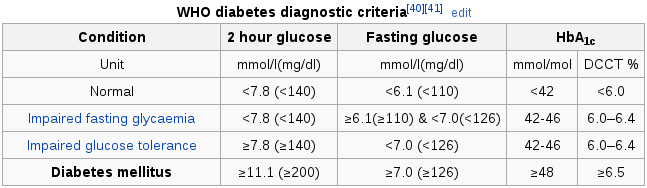
\includegraphics[width=\textwidth]{WikipediaA1CTable}
\caption{Excerpt of the Wikipedia Article on Diabetes}
\end{figure}
\section{Regular Expressions}
Modeling data is an essential part of information extraction from an unstructured data source like textual guidelines. Condition-action sentences provide information about the process flow in Clinical Guidelines. In this stage, we focus on modeling these sentences and extracting them automatically.

Condition-action sentences are not always in form of ``\texttt{if} condition \texttt{then} action''. For example, in the sentence ``Conditions that affect erythrocyte turnover and hemoglobin variants must be considered, particularly when the A1C result does not correlate with the patient's clinical situation'', we have a condition-action sentence without an ``if'' term. On the other hand, conditions may refer to effects, intentions, or events rather than activities. For instance, we see an effect of a condition in ``if the A1C is 7.0\% and a repeat result is 6.8\%, the diagnosis of diabetes is confirmed.'' We see that these sentences provide valuable information for us. So, for this stage of project, we consider them as true condition-action sentences. 

In order to identify condition-action sentences we used a simple pattern recognition by regular expressions. We consider four patterns for condition-sentences: 
\begin{itemize}
	\item `If condition, action.'
	\item `Action if condition'
	\item `When condition, action'
	\item `Action when condition'
\end{itemize}
We detected 81, 61, 62, and 60 sentences respectively, matching these patterns against the guidelines. You can see some result sentences below:

\begin{itemize}
\item Sentence: ``If adults with diabetes choose to use alcohol, they should limit intake to a moderate amount (one drink per day or less for adult women and two drinks per  day or less for  adult men) and should take extra precautions to prevent hypoglycemia. (E)''

Condition: ``adults with diabetes choose to use alcohol''

Action: ``they should limit intake to a moderate amount (one drink per day or less for adult women and two drinks per day or less for adult men) and should take extra precautions to prevent hypoglycemia.''

\item Sentence: ``When people with type 1 diabetes are deprived of insulin for 12– 48 h and are ketotic, exercise can worsen hyperglycemia and ketosis (197); therefore, vigorous activity should be avoided in the presence of ketosis.''

Condition when 1: ``people with type 1 diabetes are deprived of insulin for 12 -- 48 h and are ketotic''

Action: ``exercise can worsen hyperglycemia and ketosis -LRB- 197 -RRB- ; therefore , vigorous activity should be avoided in the presence of ketosis.''

\item Sentence: ``Metformin, if not contraindicated and if tolerated, is the preferred initial pharmacological agent for type 2 diabetes. (A)''
Condition: ``tolerated''
Action: ``is the preferred initial pharmacological agent for type 2 diabetes.''
\end{itemize}

Also we found 11, 7, 2, 5 sentences with these patterns in A1C sentences. We verified these sentences and their condition and action result manually. We observed 1 error in condition determining of A1C sentences because of existence of "," in the condition part. We also observed four faults in actions. Replacing a table with a sentence and existence of "," in condition and action segments are the reason of these faults. We achieved 80\% accuracy in identifying condition-action A1C sentences. Our accuracy for the guideline condition-action sentences is around 57\%. The decreased accuracy is the result of increasing "when" sentences, sentences with 2 conditions, sentences constructed from entire tables, and increases in sentence complexity.

To achieve classification performance with regular expressions, we need to make some changes in the preprocessing stage (such as converting table sentences to a set of well structured sentences, changing passive verbs to active verbs, splitting a complex sentence to several smaller simple sentences, etc.)

\section{Dependency Graphs}
% Integrated into Watsonsim
We aim to improve our recognition of diagnostic criteria using other knowledge also available on Wikipedia. We can do that with many of the tools we have already been developing for question answering with Watsonsim.

Firstly, rather than hard-coding the names of many diseases we want to detect, we can recognize the types of the words we encounter using answer type detection. This way our approach will generalize better for new diseases.
Secondly, we can use many Wikipedia sources to determine semantic relations between phrases. For example, we have determined that $HbA_{1c}$, as seen in the excerpt given above, is a synonym for the main article "Glycated hemoglobin." We do this by keeping a table of the redirects between Wikipedia articles. We also assume that phrases which label a link to an article are synonymous with the title of the target article, and we use this to measure synonymy.

\subsection{Lexical Answer Types}
% Tried conceptnet
% Investigating NELL
On the outset we intended to use DBPedia to detect answer types, but these are not usually specific enough to be greatly helpful, and are synonymous with the target type only on very rare occasions. We attempted to supplement this using ConceptNet, but our initial tests, before parsing the entire knowledge base, still do not indicate very high recall rates. Instead, we have developed a simple rule-based method of extracting lexical answer types from supporting passages. This covers many cases and are reasonably specific but in several instances they make unnecessary distinctions. (Sign and symptom may often be used interchangably, even though Wikipedia makes a distinction; we have noted similar situations with writer and author.) At any rate, we are examining whether to include the NELL ontology, which does at least contain many of the phrases we are targeting.

Nonetheless, there are situations where knowing the exact type of a referent is not immediately helpful. Going back to the previous example, there is no direct statement that glycated hemoglobin is a medical test in the following passage, because it is actually the subject of an implied test of its quantity:
\begin{quote}
Glycated hemoglobin (hemoglobin A1c, HbA1c, A1C, or Hb1c; sometimes also HbA1c or HGBA1C) is a form of hemoglobin that is measured primarily to identify the average plasma glucose concentration over prolonged periods of time.
\end{quote}
This is not immediately helpful because it is not yet clear that glycated hemoglobin is the subject of any test. Unless NELL or a similar ontology has this information, some other general solution for reading such tables will need to be found, or else they may need to be handled more manually.

% Could also build an ontology from reading
\subsection{Link Expansion}
When evaluating supporting passages to discover answer types, we have found it useful to annotate more than just the answer the passage supports. Finding a new object with the correct LAT but in a supporting passage for another candidate answer now triggers the generation of new candidate answers.

The intuition for such an inclusion is clear. The symptom of pain is relevant enough to diabetes for authors to choose to include it, but diabetes is not relevant enough to pain for the inverse to occur. As a result, any list of symptoms or conditions relating to diabetes will be incomplete unless the evidence for an answer comes in large part from outside of its article.

The new implications of the LAT search has the curious effect that the text analysis pipeline operates as a tree when a detected LAT suggests a new candidate. We believe we can further stimulate this effect by then running LAT detection on the newly generated candidate answers, making a pipeline a graph, but the appropriate termination conditions are as yet unclear.
% Pull pipeline
% Mention redirects
% Real links rather than redirects

\subsection{Examples and Progress}
The dependency graph approach is not complete enough to extract full conditions, though it can find symptoms and signs. For example, a query for the symptoms of diabetes will find the source text that includes the following ten symptoms for diabetes:

\medskip
\begin{tabular}{lllll}
frequent urination & increased hunger & blurry vision & 
diabetic dermadromes & fatigue \\
increased thirst & weight loss & itchy skin & slow healing of cuts & headache  \\
\end{tabular}
\medskip

The query, which is formed to imitate Jeopardy (although this soon will not be necessary), is the following: ``This symptom indicates 
diabetes:'' The suggestion apparatus adds muscle pain and thirst as symptoms, but only thirst makes the list of top ten candidate answers.

For the closely related query ``This sign indicates diabetes,'' ``Proteinuria'' is the top result, although in this case it is read from the wiki page on the symptom rather than the disease.

The query "This test indicates diabetes" discovers the type of the A1C test, and also suggests the answer "blood glucose fasting test" but later scoring does not rank the candidate very highly.
So as a result, the current recall of the LAT method is not yet more than about 10\%. The precision of answers which are actually symptoms is high but the still fewer than one in ten candidates are symptoms.

\end{document}